\section*{Łączenie wyjaśnień różnych metod}

W celu uzyskania bardziej kompleksowego zrozumienia i interpretacji modeli głębokiego uczenia, zastosowano podejście polegające na łączeniu wyjaśnień generowanych przez różne metody XAI: GradCAM, LIME i SHAP.
Łączenie wyjaśnień pozwala na wydobycie wspólnych elementów wyjaśnień, które mogą dostarczyć bardziej wiarygodnych informacji o decyzjach modelu.

W badaniach przeanalizowano dwa podejścia do łączenia wyjaśnień:
\begin{enumerate}
	\item Część wspólna - polega na wyznaczeniu wspólnych obszarów wyjaśnień generowanych przez różne metody.
	      Obszary te mogą być uznane za  bardziej pewne, ponieważ zostały wskazane przez więcej niż jedną metodę.
	\item Suma obszarów - polega na połączeniu wszystkich obszarów wyjaśnień generowanych przez różne metody.
	      Dzięki temu podejściu można uzyskać bardziej rozległe wyjaśnienia, które łączą informacje z różnych metod.
\end{enumerate}

Przeprowadzono analizę tych podejść, aby ocenić, w jaki sposób różne metody mogą być łączone, aby dostarczyć lepszych wyjaśnień decyzji modeli głębokiego uczenia.

\subsection*{Część wspólna}
Analiza części wspólnej wyjaśnień koncentruje się na identyfikacji obszarów na obrazach, które są wspólne dla metod XAI takich jak GradCAM, LIME i SHAP.
Ta metoda pozwala na odkrycie kluczowych elementów decyzyjnych modeli, które są potwierdzone przez różne techniki wyjaśniania.

\begin{figure}[h]
	\centering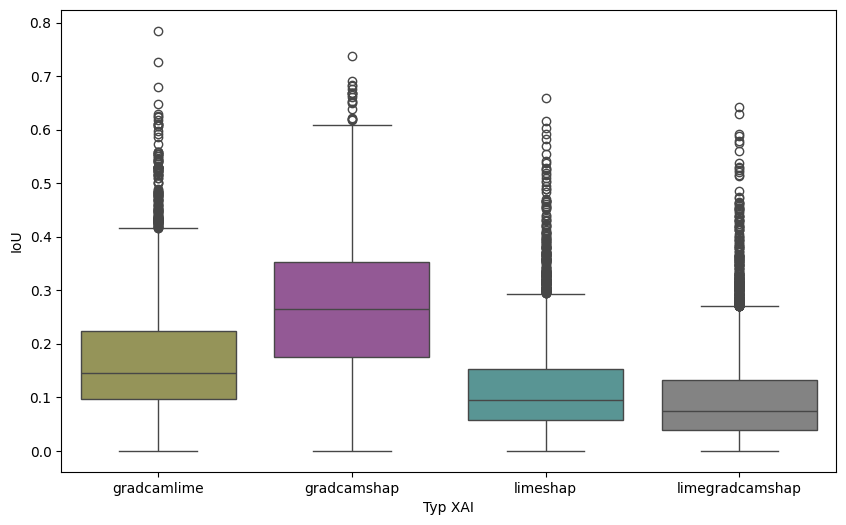
\includegraphics[width=.9\textwidth]{img/combine_iou_and}
	\caption{IoU dla połączeń wyjaśnień poprzez część wspólną}  \label{rys:combine_iou_and}
\end{figure}
\begin{table}[h]
	\centering
	\begin{tabular}{|c|c|}
		\hline
		\textbf{Metoda XAI}  & Średnie IoU \\
		\hline
		GradCAM i LIME       & 0.150297    \\
		\hline
		GradCAM i SHAP       & 0.091504    \\
		\hline
		LIME i SHAP          & 0.035271    \\
		\hline
		GradCAM, LIME i SHAP & 0.029152    \\
		\hline
	\end{tabular}
	\caption{Średnie wartości IoU części wspólnej połączonych wyjaśnień}
	\label{tab:combineandiouand}
\end{table}
Tabela \ref{tab:combineandiouand} średnie wartości dla połączonych wyjaśnień różnych metod XAI.

Najlepsze wyniki osiągnęło połączenie wyjaśnień \textbf{GradCAM} oraz \textbf{LIME}.
Najgorsze wyniki osiągnęło połączenie wszystkich trzech wyjaśnień.
Żadne z połączeń nie uzyskało lepszego średniego wyniku IoU niż średni wynik któregokolwiek z części wyjaśnień.
Powodem było zbyt duże zmniejszenie wielkość wyjaśnień.

\vspace{1cm}

\begin{figure}[h]
	\centering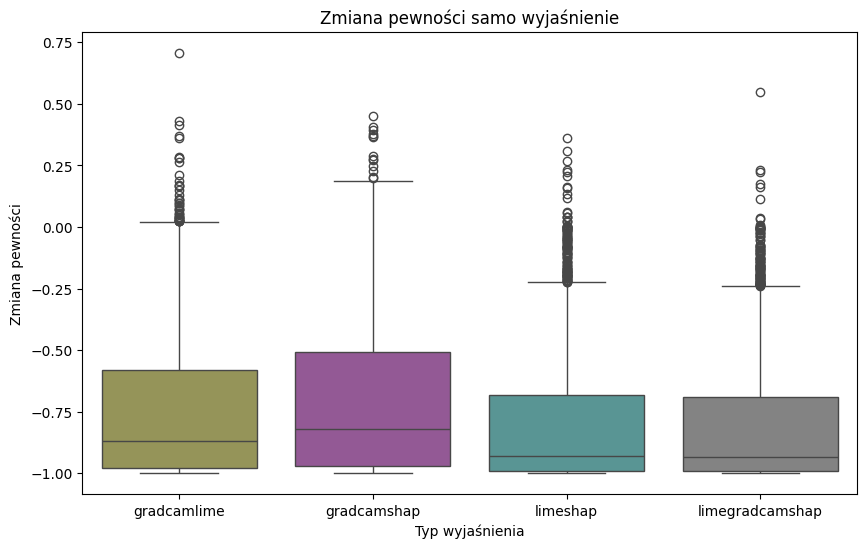
\includegraphics[width=.9\textwidth]{img/combine_confidence_exp_and}
	\caption{Zmiana pewności po pozostawieniu samego wyjaśnienia}  \label{rys:combineandconfidencean}
\end{figure}
\begin{table}[h]
	\centering
	\begin{tabular}{|c|c|}
		\hline
		\textbf{Metoda XAI}  & Zmiana pewności \\
		\hline
		GradCAM i LIME       & -0.789047       \\
		\hline
		GradCAM i SHAP       & -0.932662       \\
		\hline
		LIME i SHAP          & -0.840479       \\
		\hline
		GradCAM, LIME i SHAP & -0.789047       \\
		\hline
	\end{tabular}
	\caption{Średni spadek pewności po pozostawieniu jedynie obszaru wyjaśnienia dla części wspólnej połączonych wyjaśnień}
	\label{tab:combineandconfidenceand}
\end{table}
Zmiana pewności po pozostawieniu samego wyjaśnienia została przedstawiona na \ref{rys:combineandconfidencean} oraz w tabeli \ref{tab:combineandconfidenceand}.
Najlepsze wyniki dla połączenia \textbf{GradCAM} z \textbf{SHAP}, jednak nadal gorsze niż wyjaśnienie uzyskane z samego GradCAM lub samego SHAP.
Żadne z połączeń nie uzyskało lepszego średniego zmiany pewności niż średni wynik któregokolwiek z części wyjaśnień.

\vspace{1cm}

\begin{figure}[h]
	\centering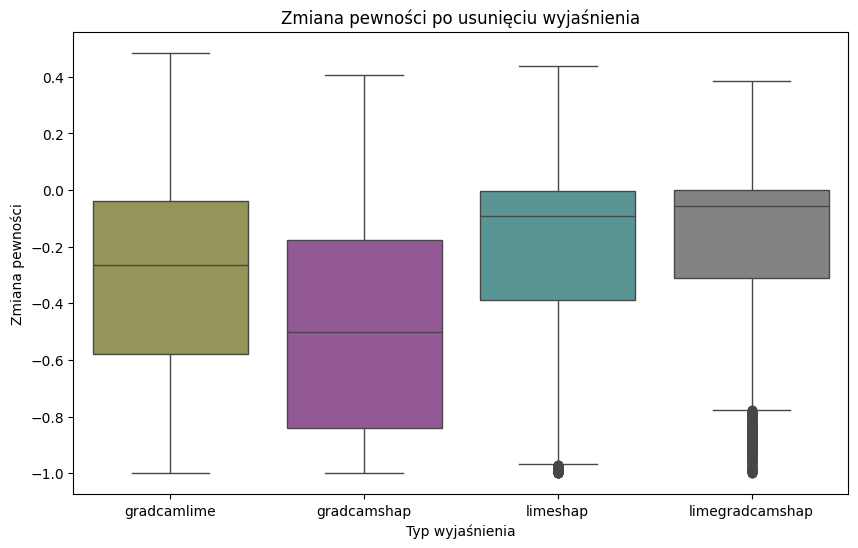
\includegraphics[width=.9\textwidth]{img/combine_confidence_no_exp_and}
	\caption{Zmiana pewności przy usunięciu obszarów wyjaśnienia}  \label{rys:combineandconfidenceandno}
\end{figure}
\begin{table}
	\centering
	\begin{tabular}{|c|c|}
		\hline
		\textbf{Metoda XAI}  & Zmiana pewności \\
		\hline
		GradCAM i LIME       & -0.290897       \\
		\hline
		GradCAM i SHAP       & -0.153363       \\
		\hline
		LIME i SHAP          & -0.068956       \\
		\hline
		GradCAM, LIME i SHAP & -0.059519       \\
		\hline
	\end{tabular}
	\caption{Średni spadek pewności modelu po usunięciu obszaru wyjaśnienia dla części wspólnej połączonych wyjaśnień}
	\label{tab:combineandconfidenceandno}
\end{table}
Zmiana pewności przy usunięciu obszarów wyjaśnienia zostały przedstawiona na rysunku \ref{rys:combineandconfidenceandno} oraz w tabeli \ref{tab:combineandconfidenceandno}
Najlepsze wyniki były dla połączenia \textbf{GradCAM} oraz \textbf{LIME}, jednak nadal gorsze niż którekolwiek z części wyjaśnień.
Żadne z połączeń nie uzyskało lepszego średniego zmiany pewności niż średni wynik któregokolwiek z części wyjaśnień.

\vspace{1cm}
Podsumowując wyjaśnienia stworzone poprzez połączenie wyjaśnień częścią wspólną, dały gorsze wyniki niż same wyjaśnienia.
Wyjaśnienia wygenerowane w ten sposób skupiają się zbytnio na małych cechach, a nie całych obiektach aby były dobrze mierzalne w tej pracy.

\subsection*{Suma obszarów}
W tej sekcji przeanalizowano, jak różne metody XAI mogą zostać połączone poprzez sumę obszarów wyjaśnień.

\begin{figure}[h]
	\centering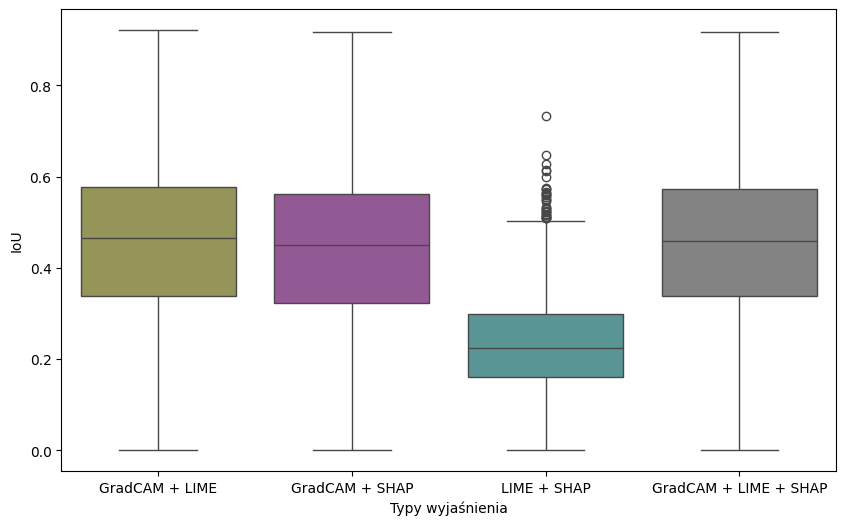
\includegraphics[width=.9\textwidth]{img/combine_iou_or}
	\caption{IoU dla połączeń wyjaśnień poprzez sumę obszarów}  \label{rys:combine_iou_or}
\end{figure}
\begin{table}[h]
	\centering
	\begin{tabular}{|c|c|}
		\hline
		\textbf{Metoda XAI}  & Średnie IoU \\
		\hline
		GradCAM i LIME       & 0.452811    \\
		\hline
		GradCAM i SHAP       & 0.438179    \\
		\hline
		SHAP i LIME          & 0.233566    \\
		\hline
		GradCAM, LIME i SHAP & 0.448209    \\
		\hline
	\end{tabular}
	\caption{Średnie wartości IoU sumy obszarów połączonych wyjaśnień}
	\label{tab:combineandiou}
\end{table}
Tabela \ref{tab:combineandiou} średnie wartości dla połączonych wyjaśnień różnych metod XAI.
Najlepszy wynik uzyskano z połączenia wyjaśnień \textbf{GradCAM} oraz \textbf{LIME}, które uzyskało wynik lepszy niż, sam GradCAM lub sam LIME.
Wszystkie połączenia dały lepsze wyniki niż dowolne jedno sani wyjaśnienie.

\vspace{1cm}

\begin{figure}[h]
	\centering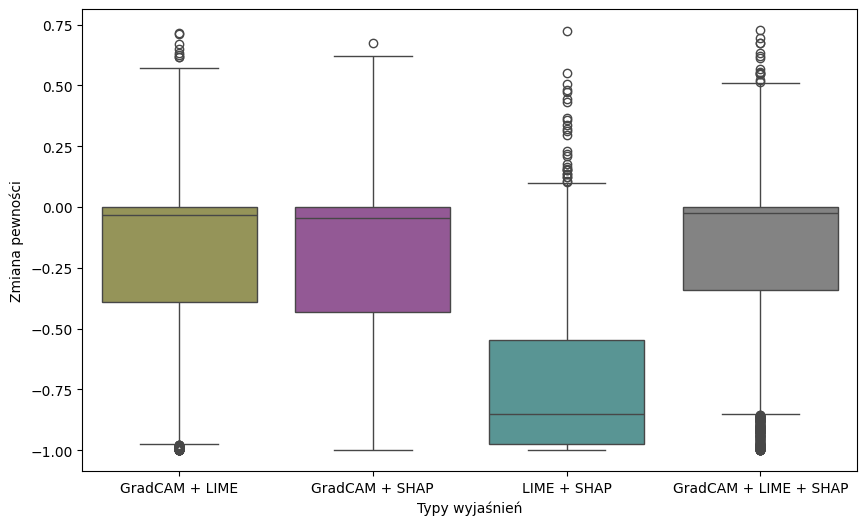
\includegraphics[width=.9\textwidth]{img/combine_confidence_exp_or}
	\caption{Zmiana pewności po pozostawieniu samego wyjaśnienia}  \label{rys:combineandconfidenceor}
\end{figure}
\begin{table}[h]
	\centering
	\begin{tabular}{|c|c|}
		\hline
		\textbf{Metoda XAI}  & Zmiana pewności \\
		\hline
		GradCAM i LIME       & -0.186505       \\
		\hline
		GradCAM i SHAP       & -0.210394       \\
		\hline
		SHAP i LIME          & -0.730767       \\
		\hline
		GradCAM, LIME i SHAP & -0.169937       \\
		\hline
	\end{tabular}
	\caption{Średni spadek pewności modelu po pozostawieniu jedynie obszaru wyjaśnienia dla sumy obszarów połączonych wyjaśnień}
	\label{tab:combineandconfidenceor}
\end{table}
Zmiana pewności po pozostawieniu samego wyjaśnienia została przedstawiona na \ref{rys:combineandconfidenceor}oraz w tabeli \ref{tab:combineandconfidenceor}.
Najlepszy wynik uzyskało połączenie wszystkich trzech wyjaśnień, co dało znacznie lepsze wyniki niż użycie jednego wyjaśnienia.
Spowodowane to było mniejszą modyfikacją.
Najgorsze wyniki uzyskało połączenie \textbf{SHAP} oraz \textbf{LIME}, nadal będąc lepszym wynikiem niż którekolwiek z pojedynczych części.
\vspace{1cm}

\begin{figure}[h]
	\centering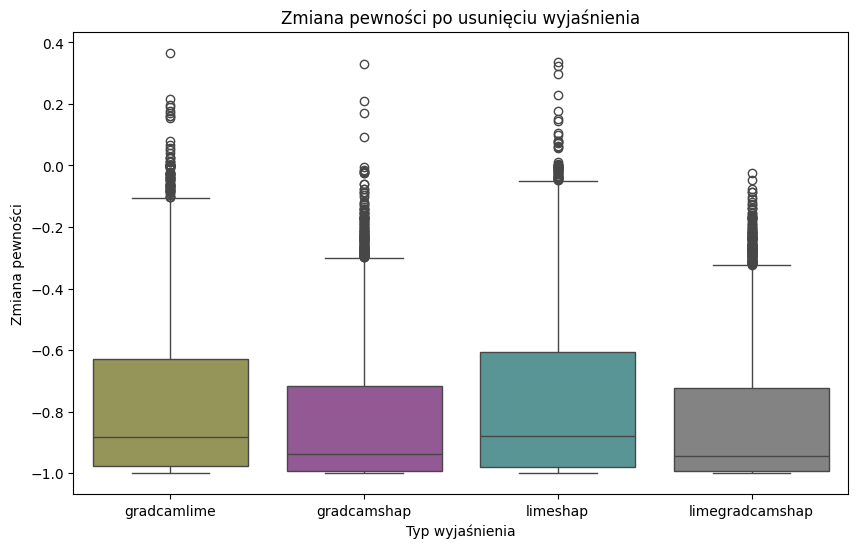
\includegraphics[width=.9\textwidth]{img/combine_confidence_no_exp_or}
	\caption{Zmiana pewności przy usunięciu obszarów wyjaśnienia}  \label{rys:combineandconfidenceorno}
\end{figure}
\begin{table}[h]
	\centering
	\begin{tabular}{|c|c|}
		\hline
		\textbf{Metoda XAI}  & Zmiana pewności \\
		\hline
		GradCAM i LIME       & -0.772289       \\
		\hline
		GradCAM i SHAP       & -0.780159       \\
		\hline
		SHAP i LIME          & -0.490221       \\
		\hline
		GradCAM, LIME i SHAP & -0.799201       \\
		\hline
	\end{tabular}
	\caption{Średni spadek pewności modelu po usunięciu obszaru wyjaśnienia dla sumy obszarów połączonych wyjaśnień}
	\label{tab:combineandconfidenceorno}
\end{table}
Zmiana pewności po pozostawieniu samego wyjaśnienia została przedstawiona na \ref{rys:combineandconfidenceorno}oraz w tabeli \ref{tab:combineandconfidenceorno}.
Najlepszy wynik uzyskało połączenie wszystkich trzech metod.
Dodatkowo tak jak wcześniej połączenie zawsze jest lepsze niż, którykolwiek element indywidualnie.

\vspace{1cm}
Podsumowując, w tych badaniach wykazano że połączenie wyjaśnień poprzez sumę pozwala na znalezienie lepszych wyników.
Kosztem takiego połączenia jest zwiększenie obszaru wyjaśnienia, wyjaśnienie tak stworzone nie jest precyzyjne.
